\chapter{Conclusões}
\label{chap:conclusoes}

Este trabalho teve como objetivo investigar a aplicação de técnicas de modelagem baseada em dados e de modelagem híbrida, com incorporação de informação física, para a predição de variáveis de desempenho em sistemas de destilação por membranas do tipo V-AGMD. O estudo concentrou-se na previsão do fluxo de permeado e das temperaturas de saída das correntes de alimentação e resfriamento a partir de variáveis operacionais do sistema, por meio de um \textit{pipeline} que integrou análise exploratória dos dados, validação cruzada com separação por regimes experimentais, comparação entre diferentes famílias de modelos e uso de predições oriundas de um modelo físico reduzido do processo.

\subsection{Conclusões gerais e interpretação dos resultados}

A partir das métricas observadas, verificou-se que o melhor desempenho para a predição do fluxo de permeado foi obtido pelo modelo híbrido ZohanResidual (RMSE 0,061), seguido pelo MLP sklearn (RMSE 0,071) e pelo HRNN (RMSE 0,078). Entretanto, para as temperaturas de saída, o modelo OLS apresentou desempenho superior (RMSE 0,246 para $T_{\mathrm{alim,out}}$ e 0,251 para $T_{\mathrm{ref,out}}$) em comparação ao ZohanResidual (RMSE 0,290 e 0,385, respectivamente). Esse resultado evidencia que os modelos híbridos, embora tenham melhorado a predição do fluxo, pioraram o desempenho para as temperaturas de saída.

Esse comportamento pode ser atribuído a dois fatores principais. Primeiro, o critério de seleção de hiperparâmetros priorizou exclusivamente o RMSE do fluxo de permeado, sem considerar o impacto dessa escolha sobre as demais variáveis de saída. Segundo, as análises exploratórias indicaram que as temperaturas de saída apresentam relações aproximadamente lineares com as variáveis de entrada (conforme evidenciado pelos coeficientes de Pearson e Spearman e pelos gráficos de dispersão), enquanto o fluxo de permeado exibe dependência mais complexa e multivariada. Dessa forma, a região operacional analisada parece estar contida em um domínio aproximadamente linear para as variáveis térmicas, favorecendo modelos mais simples como a regressão OLS.

A performance competitiva das famílias de modelos lineares sugere que, na faixa operacional analisada, uma parcela relevante da variabilidade dos alvos pode ser representada por relações de menor complexidade. Ainda assim, o ganho obtido pelo modelo híbrido para o fluxo indica que a representação não linear da rede neural, combinada à informação física fornecida pelo modelo 0D, permitiu capturar efeitos adicionais associados ao acoplamento entre transferência de calor e massa no processo.

A Figura~\ref{fig:best_per_family_rmse} apresenta a comparação de desempenho entre os melhores modelos de cada família, evidenciando o trade-off entre a predição do fluxo e das temperaturas. O modelo OLS destaca-se pelo melhor equilíbrio entre as três variáveis, enquanto o ZohanResidual concentra seu ganho no fluxo de permeado.

\begin{figure}[H]
    \centering
    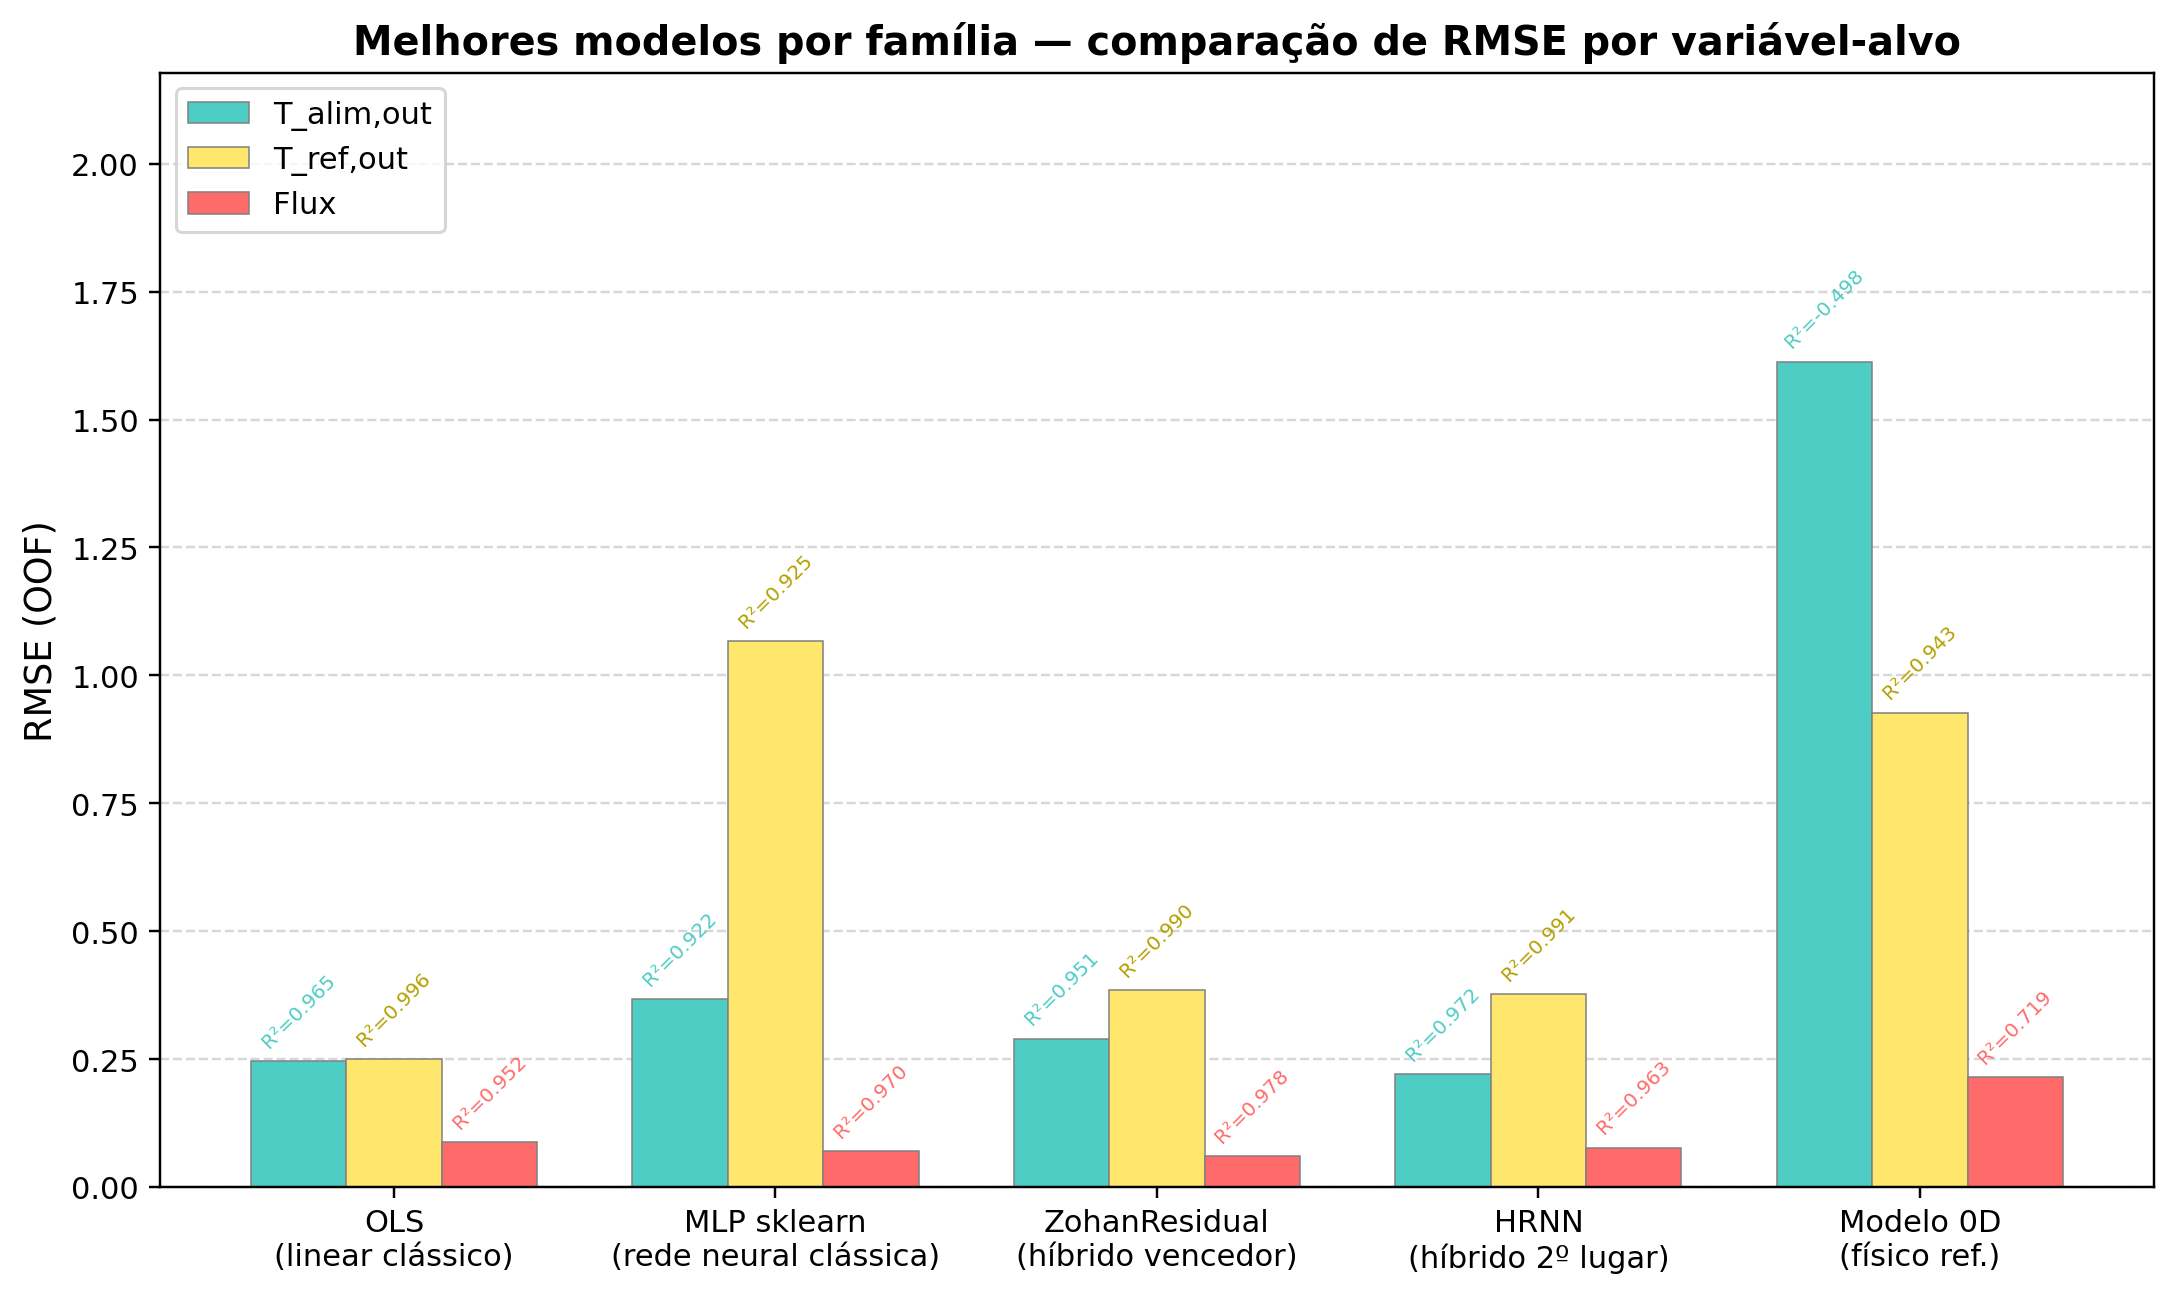
\includegraphics[width=0.85\textwidth]{Imagens/chap06/best_per_family_rmse.png}
    \caption[Comparação de RMSE entre melhores modelos de cada família]{Comparação do RMSE entre os melhores modelos de cada família para as três variáveis de saída. O modelo OLS apresenta o melhor desempenho para as temperaturas de saída, enquanto o ZohanResidual é superior para o fluxo de permeado.}
    \label{fig:best_per_family_rmse}
    \fonte{Elaborado pela autora.}
\end{figure}

Do ponto de vista conceitual, esse resultado pode ser interpretado como uma aproximação de um cenário ideal de modelagem híbrida. O modelo mais adequado para representar o comportamento do sistema seria aquele capaz de reproduzir, de forma eficiente, as equações de balanço de massa e energia e, simultaneamente, incorporar as imperfeições observadas na operação real. Nesse sentido, a estratégia adotada se aproxima desse objetivo ao combinar as predições do modelo físico reduzido com uma rede neural treinada para aprender correções sistemáticas em relação aos dados experimentais.

Sob essa perspectiva, a rede neural fornece uma estrutura capaz de aproximar relações não lineares complexas, enquanto o modelo físico 0D representa, de forma simplificada ou média, os principais acoplamentos fenomenológicos do sistema. A combinação dessas duas abordagens permite que o modelo híbrido incorpore tanto a informação empírica presente nos dados quanto uma tendência física previamente estimada pelo modelo fenomenológico. No entanto, essa aproximação permanece limitada à região de operação contemplada pelos dados experimentais. Assim, mesmo com a incorporação de informação física, a capacidade de generalização do modelo continua dependente da cobertura dos dados disponíveis e não deve ser interpretada como garantia de extrapolação para condições operacionais não avaliadas experimentalmente.

Essa interpretação é particularmente relevante porque o modelo físico reduzido está sujeito a simplificações inerentes à sua formulação. Assim, a rede híbrida atua como um corretor sistemático das discrepâncias entre o modelo físico e o comportamento experimental. Essa complementaridade mostrou-se mais eficaz do que o uso isolado de modelos puramente \textit{data-driven} ou puramente \textit{physics-driven}, ao menos dentro da faixa de operação investigada.

A análise também deve considerar os fundamentos estatísticos da capacidade de generalização. Modelos mais flexíveis podem apresentar excelente ajuste ao conjunto de treinamento sem necessariamente reproduzir novos dados com precisão, especialmente na presença de ruído experimental. Nesse trabalho, o uso de validação cruzada e critérios de seleção com penalização de complexidade foi fundamental para reduzir o risco de sobreajuste. O bom desempenho do modelo ZohanResidual sugere que sua maior flexibilidade foi adequadamente regularizada, permitindo capturar relações consistentes nos dados.


Além disso, as diferentes variáveis de saída estão fisicamente acopladas. O fluxo de permeado depende diretamente dos gradientes térmicos e de pressão de vapor estabelecidos no módulo, bem como das resistências térmicas e difusivas e dos efeitos de polarização. Ao mesmo tempo, as temperaturas de saída também são afetadas pela transferência de massa, uma vez que a evaporação e a condensação do permeado envolvem trocas de calor latente e alteram os balanços de energia nas correntes de alimentação e refrigeração. Assim, embora a seleção de modelos tenha sido orientada prioritariamente pelo erro associado ao fluxo de permeado, a previsão das temperaturas permanece como uma avaliação relevante da capacidade do modelo em representar o comportamento térmico acoplado do sistema.

Entretanto, os resultados indicam que, devido à priorização exclusiva do fluxo no critério de seleção, as temperaturas de saída foram prejudicadas nos modelos híbridos. Enquanto a OLS obteve RMSE de 0,246 para $T_{\mathrm{alim,out}}$, o modelo ZohanResidual elevou esse erro para 0,290. Isso sugere que o modelo recomendado para a predição do fluxo de permeado e para as temperaturas de saída são distintos: modelos lineares simples (como OLS) são preferíveis para as temperaturas, enquanto os híbridos (ZohanResidual) são superiores para o fluxo.

Destaca-se que a estratégia de seleção de modelos foi deliberadamente orientada pela previsão do fluxo de permeado, por este representar o principal indicador de produtividade do processo. Embora todos os modelos tenham sido treinados para prever simultaneamente o fluxo e as temperaturas de saída, a busca e a seleção de hiperparâmetros utilizaram como critério principal o erro associado ao alvo $Flux$. Esse procedimento não foi repetido separadamente para $Alim\_T\_out$ e $Ref\_T\_out$, a fim de manter uma única estratégia de seleção alinhada ao objetivo central do trabalho.

Ainda assim, as temperaturas de saída foram mantidas na avaliação por sua relevância física e energética. O contraste entre o desempenho para fluxo e temperaturas abre uma direção importante para trabalhos futuros: a realização de buscas de hiperparâmetros com funções objetivo multi-resposta, nas quais pesos diferenciados sejam atribuídos a cada variável de saída, ou a seleção de modelos distintos para cada alvo.

\subsection{Trabalhos futuros}

A partir dos resultados obtidos, diversas possibilidades de aprofundamento podem ser propostas.

Uma primeira direção consiste em investigar estratégias de modelagem que priorizem explicitamente a predição das temperaturas de saída, seja por meio de funções objetivo multi-resposta com pesos diferenciados, critérios de seleção orientados por erro térmico ou buscas de hiperparâmetros dedicadas a essas variáveis. Idealmente, seria interessante realizar novas rodadas do \textit{pipeline} de regressão com pesos alterados entre as variáveis na função de escolha, permitindo que o modelo selecionado reflita um compromisso customizável entre fluxo e temperaturas.

Uma segunda linha envolve o refinamento da incorporação de conhecimento físico. Uma abordagem promissora seria o uso de \textit{Physics-Informed Neural Networks} (PINNs) para criar uma rede \textit{surrogate} que implemente as equações diferenciais do processo (sem as simplificações do modelo 0D) e possa substituir a coluna \texttt{phy} utilizada neste trabalho. Essa PINN poderia então ser empregada como referência física de maior fidelidade na hibridização com os dados experimentais, potencialmente melhorando a predição de todas as variáveis de saída.

Outra linha de investigação promissora envolve o uso de \textit{Physics-Informed Neural Networks} (PINNs), as quais podem ser exploradas sob duas perspectivas complementares. A primeira consiste em uma formulação com função de perda híbrida, combinando o erro em relação aos dados experimentais com um termo de regularização física baseado nas equações governantes do processo, de modo a restringir as soluções a regiões fisicamente admissíveis. A segunda perspectiva envolve o treinamento de uma PINN exclusivamente a partir de dados sintéticos gerados pelo modelo físico 0D, permitindo que a rede aprenda o comportamento fenomenológico do sistema sem depender diretamente de dados experimentais. Nesse caso, a PINN treinada poderia substituir o próprio modelo 0D como base para as arquiteturas residuais híbridas, oferecendo um substituto computacionalmente mais eficiente e potencialmente mais flexível.

Alternativamente, poder-se-iam inserir os dados experimentais diretamente no treinamento da PINN. No entanto, a região operacional disponível parece estar contida em um domínio aproximadamente linear, conforme indicado pelo bom desempenho de modelos de regressão linear e pelos coeficientes de correlação. Isso sugere que os dados experimentais cobrem uma faixa limitada do espaço de operação, o que deixaria lacunas significativas no treinamento de uma PINN. Nesse contexto, a estratégia de gerar um \textit{surrogate} para popular a coluna \texttt{phy} e, simultaneamente, investigar maneiras de criar uma \textit{baseline} neural mais robusta para os modelos híbridos constitui uma metodologia promissora para melhorar o desempenho preditivo em sistemas de destilação por membranas.

Além disso, seria relevante realizar uma busca de hiperparâmetros dedicada exclusivamente às temperaturas de saída, uma vez que este trabalho priorizou apenas o fluxo de permeado. A partir dessa busca, poderia-se implementar uma rede \textit{surrogate} baseada em EDOs (sem as simplificações do modelo 0D atual) acoplada a uma \textit{baseline} otimizada, criando um arcabouço de modelagem híbrida mais completo e preciso.

Uma ampliação natural deste trabalho consiste na obtenção de novos dados experimentais em regiões mais amplas do espaço de operação. Isso permitiria avaliar a robustez dos modelos fora da região atualmente analisada e explorar de forma mais clara possíveis não linearidades do sistema.

Por fim, os modelos desenvolvidos podem ser aplicados em estudos de otimização operacional, permitindo identificar condições de operação que maximizem a produtividade, minimizem o consumo energético ou conciliem ambos os objetivos.

Ressalta-se que o \textit{pipeline} desenvolvido neste trabalho é agnóstico em relação ao sistema físico de origem: o mesmo arcabouço metodológico — desde a estruturação dos dados com separação por grupos, passando pela validação cruzada e seleção hierárquica de modelos, até a incorporação de informação física via arquiteturas híbridas — pode ser aplicado a qualquer conjunto de dados de entrada e saída. Isso torna a metodologia proposta potencialmente relevante para uma ampla gama de problemas de engenharia nos quais se deseje combinar modelagem fenomenológica com aprendizado a partir de dados experimentais.

Em síntese, este trabalho mostrou que a integração entre modelos físicos reduzidos e aprendizado de máquina constitui uma abordagem eficaz para a modelagem de sistemas V-AGMD. Os resultados reforçam que a combinação entre conhecimento fenomenológico, validação estatística rigorosa e estratégias de modelagem híbrida é fundamental para obter modelos preditivos robustos, interpretáveis e relevantes do ponto de vista de engenharia.